\documentclass{article}
% The file ijcai11.sty is the style file for IJCAI-11 (same as ijcai07.sty).
\usepackage{ijcai11}

% Use the postscript times font!
\usepackage{times}
\usepackage[utf8x]{inputenc}
\usepackage{datetime}
\usepackage{graphicx}
\usepackage{dblfloatfix}
%\usepackage{stfloats}
\usepackage{mathptmx}
\usepackage[T1]{fontenc}

% the following package is optional:
\usepackage{latexsym}

% Following comment is from ijcai97-submit.tex:
% The preparation of these files was supported by Schlumberger Palo Alto
% Research, AT\&T Bell Laboratories, and Morgan Kaufmann Publishers.
% Shirley Jowell, of Morgan Kaufmann Publishers, and Peter F.
% Patel-Schneider, of AT\&T Bell Laboratories collaborated on their
% preparation.

% These instructions can be modified and used in other conferences as long
% as credit to the authors and supporting agencies is retained, this notice
% is not changed, and further modification or reuse is not restricted.
% Neither Shirley Jowell nor Peter F. Patel-Schneider can be listed as
% contacts for providing assistance without their prior permission.

% To use for other conferences, change references to files and the
% conference appropriate and use other authors, contacts, publishers, and
% organizations.
% Also change the deadline and address for returning papers and the length and
% page charge instructions.
% Put where the files are available in the appropriate places.


\title{Master 1 MoSIG Research Project Report\\
Learning Job Runtimes in HPC Systems}
\author{Valentin Reis\\
  Supervised by: Denis Trystram \& Eric Gaussier.\\
}

\begin{document}

\maketitle

{% Mosig student
  {\hbox to0pt{\vbox{\baselineskip=10dd\hrule\hbox
        to\hsize{\vrule\kern3pt\vbox{\kern3pt
            \hbox{{\small I understand what plagiarism entails and I declare that this report }}
            \hbox{{\small is my own, original work. }}
            \hbox{{\small Name, date and signature: }}
            \kern3pt
          }\hfil%\kern3pt
          \vrule
      }\hrule}
  }}
}


\begin{abstract}
  In many HPC infrastructures, the descriptions of the tasks to be executed are subject to high uncertainty. We show that users are unreliable when estimating the run time of their jobs, and look into alternative solutions. Predictive techniques are investigated in order to infer the run time of jobs from their full description and system history. A Machine Learning technique, Random Forests is applied and compared against the state of the art. We show that the prediction obtained with this approach has good properties with respect to relevant metrics.
\end{abstract}

\section{Introduction}
High Performance Computing (HPC) systems are complex machinery at the frontier between research in scheduling and systems engineering. We outline two of the main difficulties that resource management software in this field have to face.

First, the ephemeral nature, and broad range of existing architectures of those systems make the development and application of theoretical results difficult.
New schemes for distributing resources are more present than ever. Many recent systems have complex network and memory/hard drive sharing topologies. Moreover, the topology of HPC systems can now change on a hourly to monthly basis, since the hardware of distributed systems can be reconfigured or extended continually.
Finding scheduling and resource management strategies which can deal with complex systems and adapt to their evolutions poses a challenge.

In addition, the data (i.e.\ the characteristics of the tasks to be executed) these systems have to work with presents many peculiarities.
The nature of the information which users of the system provide is very often loose, by instance with only upper and/or lower bounds on numerical quantities provided.
For instance, and this will be the focus of this paper, the run time of a given job on a specific system is seldom known in advance, but many cluster management software ask the users for an upper bound on this quantity.

As a consequence of these difficulties most free, open-source and commercial resource management software use simple heuristics that can provide bounds on their performance and/or guarantee a few functional properties.
An example of such a heuristic is the First Come First Serve (FCFS) policy to schedule parallel jobs on a homogeneous cluster of machines, which starts jobs as soon as possible, in the exact order they were submitted.
Among other properties ,such as robustness to lack of information about the amount of time jobs will run on the system, this strategy guarantees the avoidance of starvation.

\subsection{Research Direction}
The general direction we are headed in with this research project is to deal with the input data of the resource management systems.
Accommodating for this data seems separable enough from the actual scheduling problems for work towards this objective to be rewarding.
No innovative ways to query the data from the users will be studied, we will rely on existing logs from HPC systems. Instead, we seek to apply Machine Learning(ML) techniques in order to reduce uncertainty of, and extract information and/or structure from, the input data of the HPC systems.
We will be working with the problem of presenting input data in the most valuable way possible to a scheduling algorithm. How to use this data to the fullest will not be discussed.
When assessing the relevance of the specific information we choose to produce from the job characteristics, references from the scheduling literature and existing systems will provide ground to stand on.


\begin{figure*}[b]
  %\centering\rule{0.8*\textwidth}{0.3*\textwidth}
  \centering
  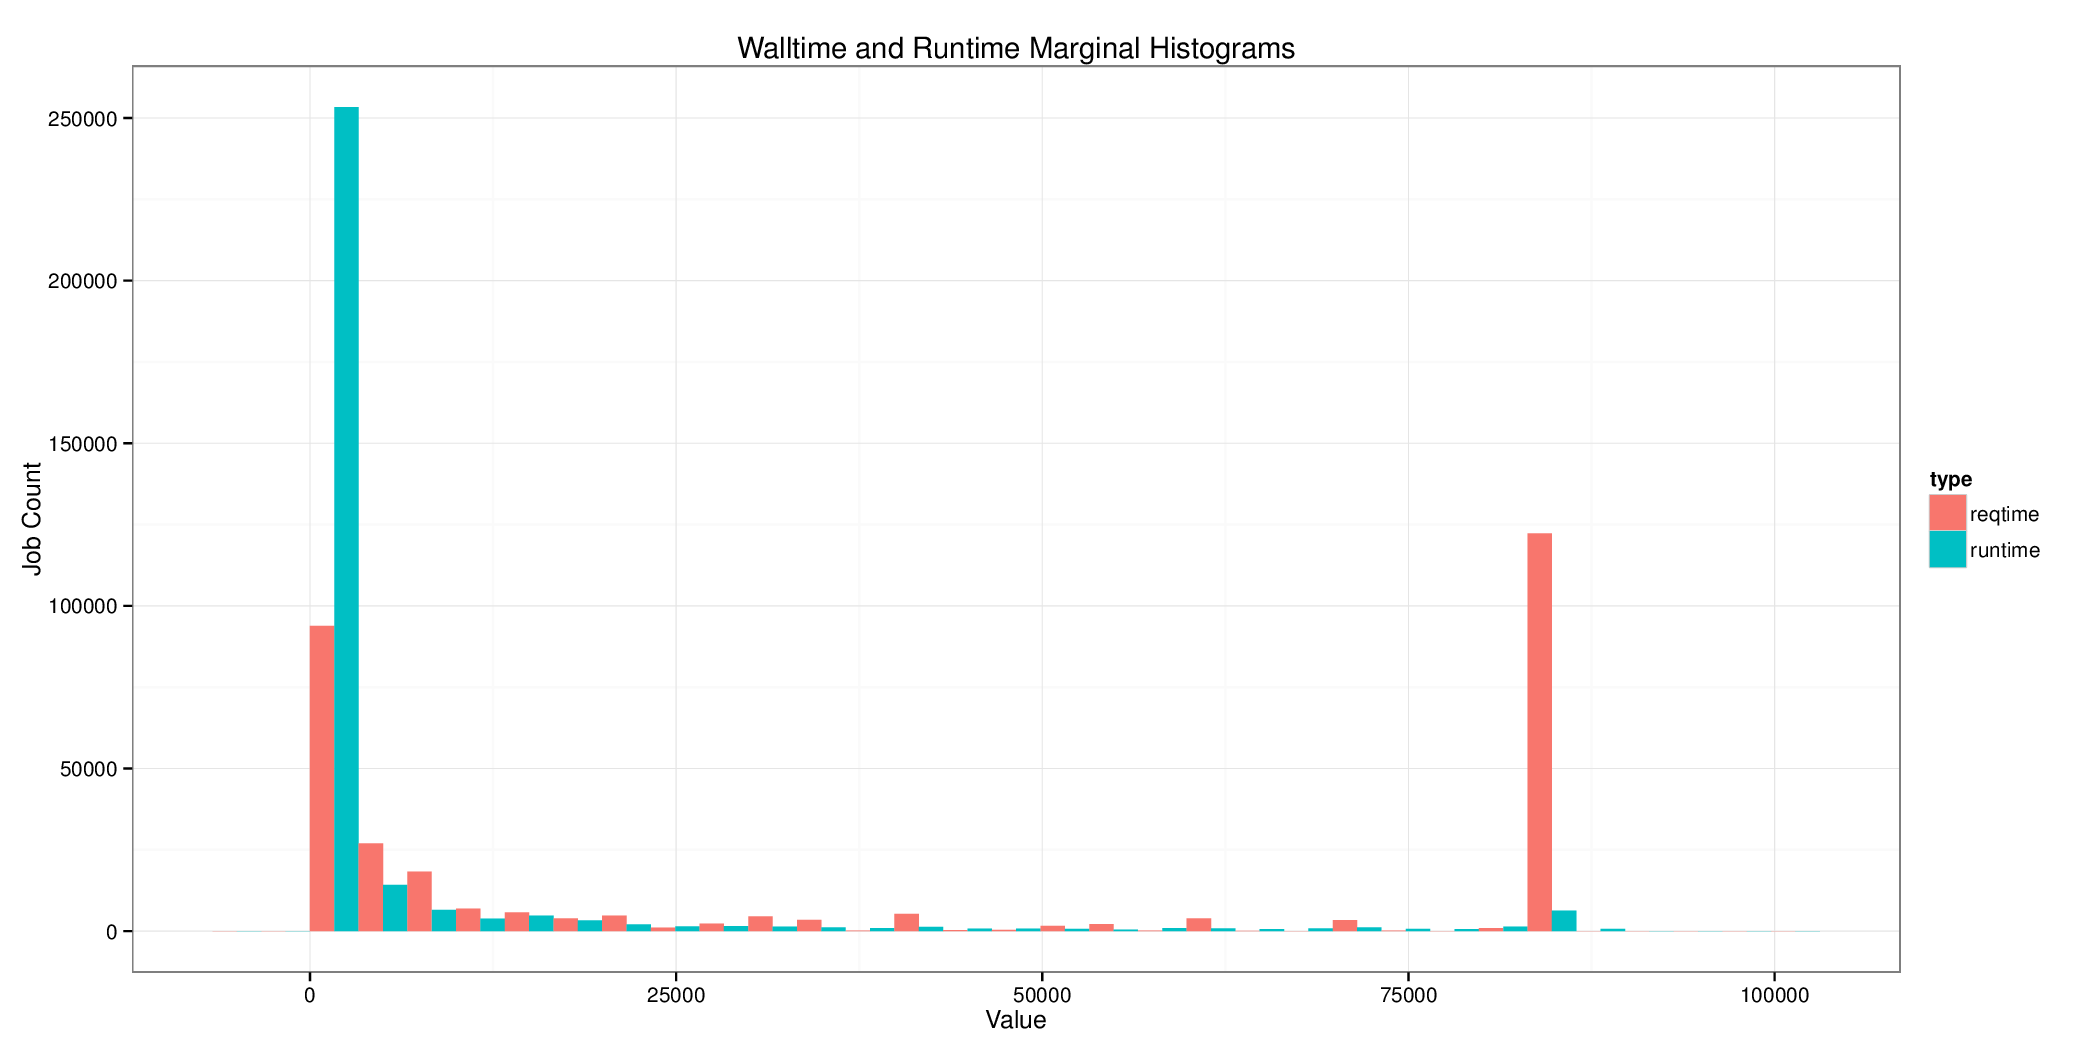
\includegraphics[width=\textwidth]{../../wallimage-0.png}
  \caption{Marginal Histograms of the \textbf{reqtime} and \textbf{runtime} of all jobs from the CEA CURIE log.}
  \label{fig:_wall_run_for_report_pdf}
\end{figure*}



\begin{figure*}[b]
  \centering
  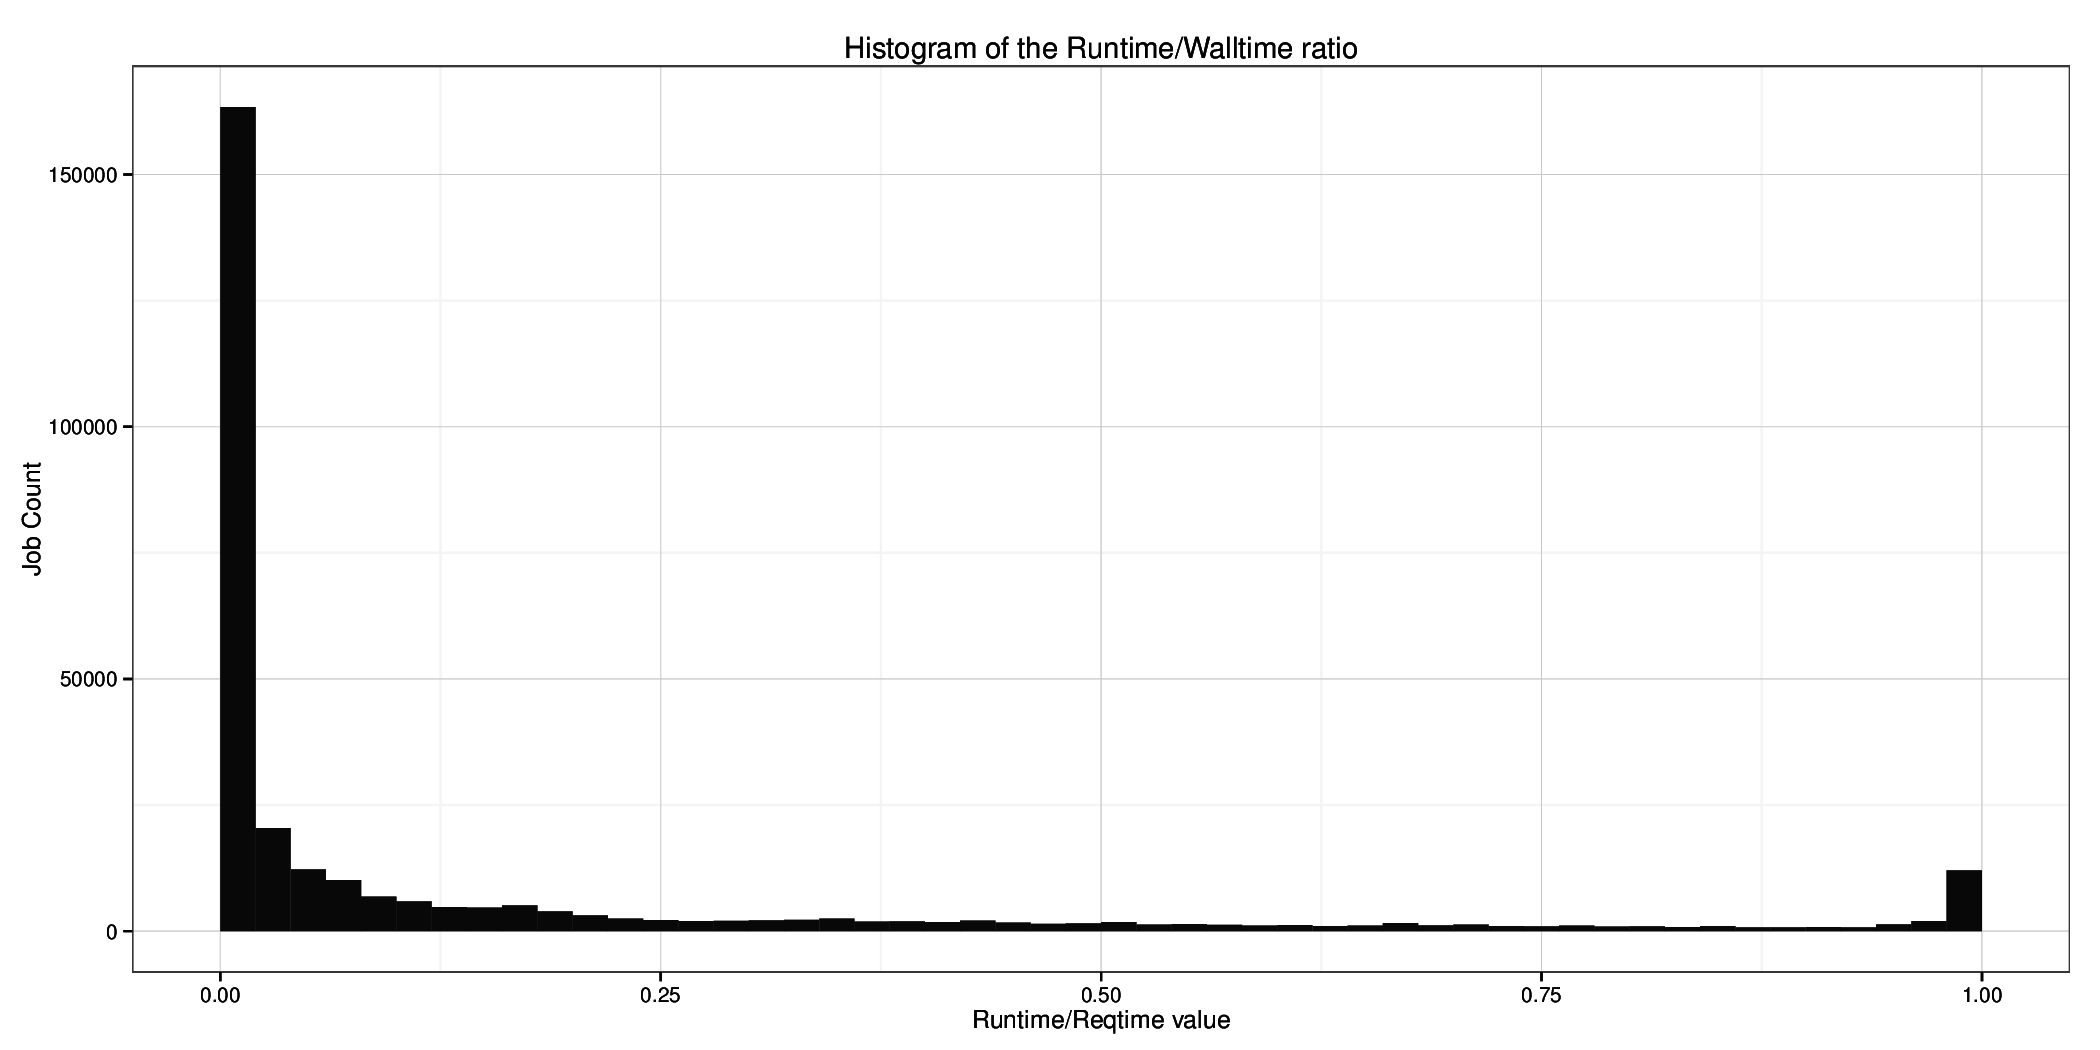
\includegraphics[width=\textwidth]{../../wallimage-1.png}
  \caption{Histogram of the $\frac{\textbf{runtime}}{\textbf{reqtime}}$ ratio in the CURIE log.}
  \label{fig:ratio}
\end{figure*}

\subsection{Job runtimes}
Most HPC resource management software (including the SLURM, OpenPBS, OpenLava and OAR software) do ask information about jobs to users, such as topological requests in terms of processing units and memory, the name of the executable, miscellaneous functional requirements and, last but not least, the expected run time of the job with respect to its hardware requirements.
This user-provided estimate of the run time of a job on a specific system will be referred as \textbf{reqtime} in the rest of the paper. Most of these software use the \textbf{reqtime} of a job as an upper bound on its run time, and kill it should \textbf{reqtime} be violated. As a consequence, users overestimate this value, should they choose or be forced to provide it. The following section will present a statistical analysis pertaining to this relationship.

The true run time of a job with respect to a given affected topology is of great interest, as the scheduling policies are highly dependent on this information to provide good solutions \~ref{truc}. We will refer to this quantity as the \textbf{runtime} of a job.
It must be clear that in the context of topological heterogeneity, the \textbf{runtime} of a job is only defined with respect to a specific processing environment to which it might be affected.
This can include, and is not limited to, the network topology of the processing units, the availability of shared memory, message passing costs, and the operating system supporting the computations.

\subsection{Problem Statement}
In this paper, the broad question of refining the data is reduced to a single variable, the \textbf{runtime}. The problem statement we are dealing with is the following.

Given a specific homogeneous HPC Cluster with negligible communication costs, how to best predict the value of the \textbf{runtime} of a job?

The choice of dealing with homogeneous distributed machines without communication costs in a first approach has the interesting property of separating the data treatment from the scheduling and interaction with the system.
In this case, the \textbf{runtime} becomes an intrinsic attribute of a job.
On the contrary to the input data which is always subject to peculiarities of the various systems and software, the \textbf{runtime} is always present as a simple field in workload logs of HPC systems, such as those available at the workload archive ~\cite{workloadarchive}.

This problem statement implies a latent question: How to communicate the prediction to the rest of the system (e.g.\ single-value, probability density, confidence factor)? Alternatives will be discussed but ultimately, the focus will be on single-valued predictions.
As mentioned previously, our approach is to use machine learning techniques. We will be inferring runtime from the job characteristics by learning from system logs, and since this is a value in $[0,+\infty ]$, this is a supervised learning problem, namely regression.

We will be careful to only learn our models on logs from homogeneous systems, or homogeneous subsets of systems which are sizeable enough to learn from.
As for downplaying the impact of communication costs, we will further restrict our work to machines which do not possess overly complex topology or distribute computing nodes across more than a handful of routers.
In essence, we are targeting large Beowulf clusters, supercomputers, GPU farms and mainframe clusters.

\section{Motivation}

\subsection{Importance of \textbf{runtime}}
\label{sub:importance_of_runtime}
Once again, we emphasise the role of the \textbf{runtime} in scheduling tasks. Virtually all results from scheduling theory use the `clairvoyant' model~\cite{handbook-of-scheduling}, where \textbf{runtimes} of jobs with respect to all possible affectations on the system are known in advance.
%TODO: ref clairvoyant? ok?
Intuitively, in order to use this extensive theoretical body, we would need to reduce uncertainty in this variable.
%TODO:ref Denis FCFS wait? ok?
It has been shown~\cite{tsafir} that even in the classical approach (which is to use policies that are robust to this uncertainty), there is added value when this variable is refined.
In all cases, reducing uncertainty in \textbf{runtime} is critical to the success of the approach used to schedule jobs.

As mentioned before, existing solutions use much simpler heuristics. We will now focus on a particular system in order show why a simple scheduling heuristic is applied.
% subsection importance_of_runtime (end)

\subsection{Reqtime vs Runtime on a real system}
\label{sub:reqtime_vs_runtime_on_a_real_system}
The following study is conducted on a log[ref log] containing 20 months worth of data from the CURIE[ref curie] supercomputer operated by the French government-funded research organization CEA (Commissariat à l'Énergie Atomique).
It contains more than 300,000 jobs, submitted from February 2011 to October 2012 by 900 users in the `cleaned' version from the workload archive~\cite{workloadarchive}.
The log has several homogeneous CPU partitions and CPU+GPU partitions, however in a each partition, all nodes are identical.
Jobs are allocated to partitions using user preference. The system is managed using the SLURM (Simple Linux Utility for Resource Management) software.
Figure~\ref{fig:_wall_run_for_report_pdf} shows the marginal distributions of \textbf{reqtimes} and \textbf{runtimes} on this system. The marginal distributions are already revealing, we can see that many \textbf{reqtimes} are in the 24h bin.
The reason for this is that 24h is both the maximal value and the default one: on this system, users may choose not to provide an estimate for their job's \textbf{runtimes}, in which case the maximum value is used by the scheduler.
Further looking into the relationship between reqtime and runtime, Figure~\ref{fig:ratio} shows how the ratio $\frac{\textbf{runtime}}{\textbf{reqtime}}$ is distributed. This histogram indicates that a majority of users either: have very little idea about the expected \textbf{runtime} of their jobs, or overestimate very strongly its value on purpose. Sophisticated scheduling methods are not applied: under such uncertainty in the \textbf{runtime},  their performance is equivalent to the simple heuristic which is applied, namely FCFS with Backfilling~\cite{backfilling}.
% subsection reqtime_vs_runtime_on_a_real_system (end)

\section{State of the art in \textbf{runtime} prediction}

As mentioned previously, the latent question when predicting the \textbf{runtime} is how to provide the information to the scheduling algorithm. This section presents a few alternatives and state of the art methods in each case.

\begin{figure*}[b]
  \centering
  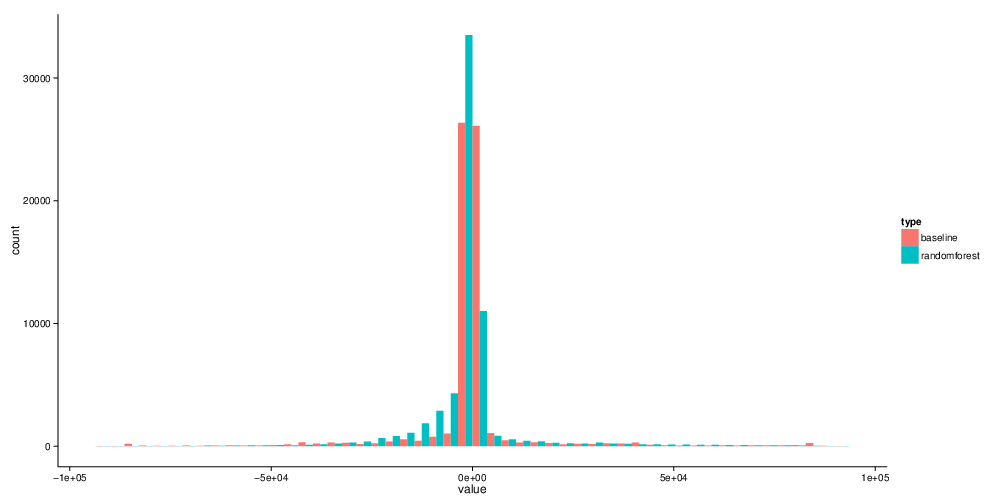
\includegraphics[width=\textwidth]{../../truc.png}
  \caption{Histogram of the error made in the predictionfor both the baseline and random forest methods, on the 20\% of the last jobs of the CURIE dataset.}
  \label{fig:ratio}
\end{figure*}


\subsection{Predicting a value}
\label{sub:predicting_a_value}

Predicting values has been first attempted~\cite{gibbons} by binning jobs in a predefined partitioning of their feature space and averaging values in each bin to provide an estimate. In this method, the partitionning has to be provided by the Resource Management Software or the system administrator. This method assumes the data to be identically distributed and independent. It does not make use of dependency between successive jobs. Moreover, the binning has to be obtained trough careful statistical analysis of the specific system and population.

A more simple approach~\cite{tsafir} averages the two last available runtimes of the job's user.
This method makes full use of the dependency between successive runtimes, but does not make use of the jobs's description. Its main selling point are it's simplicity and accuracy.

% subsection predicting_a_value (end)

\subsection{Predicting a distribution}
\label{sub:predicting_a_distribution}

An algorithms that uses a probability distribution of single job runtimes~\cite{probabilistic-backfilling} have been proposed, with an accompanying distribution prediction tool~\cite{hmm}. This tool is similar to the previous method of averaging the two previous runtimes for the job's user, in the sense that it only relies on the runtime information. It treats successive runtimes of a given user as the observations of a Hidden Markov Model~\cite{rabiner}. It does not use the job description.

% subsection predicting_a_distribution (end)
\section{A Regression Approach}
\label{sec:our_approach}
We make the observation that single job runtime prediction might be improved by using both the `runtime locality' (i.e.\ the dependency between successive runtimes) and the job features. We will experiment with a method that will allow us to bridge this gap.
The chosen method is to perform regression on vectors containing the following features:
\begin{itemize}
  \item The continuous and discrete attributes from the job's description, such as \textbf{reqtime}, number of cores required,or time of the day of the sumbission.
  \item The attributes of the last $n$ jobs of this user, where $n$ is to be chosen as to balance between the cost of fitting the model and its accuracy.
  \item Attributes from the user and the system, such as the amount of nodes the user is currently using on the system, or the mean runtimes of jobs of the user.
  \item Predicted values which come from other techniques, such as averaging the two previous runtime values.
\end{itemize}
This approach has the advantage of being rather adaptable to various formulations of the job description.
No two HPC systems are identical, therefore this provides a clear added value, as it is now the algorithm's responsibility deal with the particularities of the input data on each system.
It is however difficult to provide validation of this aspect of the specific algorithm we will use, and this will not be in the scope of this paper.

\subsection{Random Forests}
\label{sub:random_forests}
The specfic ML algorithm we use is called Random Forests, and in particular the CART~\cite{randomforest} method.
This technique is an ensemble learning method based upon Decision Tree Learning~\cite{decisiontrees}.
Decision Trees partition the feature space: in a tree, the splitting is performed by using a threshold for continuous features and a all-way split on categorical features.
Decision Trees are usually learned on a training set with a recursive top-down greedy algorithm which optimizes a function of the tree and the training set.
Such a function can be for instance the Information Gain~\cite{kullback} of the tree on the training set. A criterion on the purity of leaves and/or amount of vectors which fall therein is used to stop the construction. Training set real output values are then averaged in each leaf to give predictions: When regressing a data point, it is sent trough the tree and the algorithm outputs the value of the corresponding leaf.
The CART algorithm functions in the following manner:
\begin{itemize}
  \item Training: \begin{itemize}
      \item Randomly partition the training data.
      \item Build decision trees on each partition.
    \end{itemize}
  \item Predict a value by combining (e.g.\ average or linear combination) the results from all the trees.
\end{itemize}
% subsection random_forests (end)

\subsection{Interpretation of the model}
\label{sub:explainability}
This approach has the advantage of producing an explainable model.
Nodes which are, on average, higher up the decision trees are more important in the decision process.
By ranking input vector attributes according to their average height in the trees, we will be able to gain insight about which feature is the most crucial to predicting the runtime.
However, given the important height and complexity of the trees, it is hard to produce more information.
There exist techniques ~\cite{interpret} to interpret further the model, however they are not implemented in the free and open-source Random Forest packages, and we did not use them due to time constraints.
% subsection interpretation of the model (end)

% section our_approach (end)

\section{Preliminary Results}
\label{sec:preliminary_results}
We run the CART algorithm on a dataset built from the CURIE log which was analyzed in~\ref{sub:reqtime_vs_runtime_on_a_real_system}. In a first approach, we choose to validate our approach by training the algorithm with the first 80\% of the job/runtime associations and predicting the last 20\% of the runtimes. We then compare our results with an existing popular baseline, namely averaging the two last available runtime values from the job user~\cite{tsafir}, in order to validate our method.

\subsection{Feature List}
\label{sub:feature_list}
Figure~\ref{fig:features} shows the exact data vectors we use when running the random forests.

\begin{figure}[!ht]
  \centering
  \begin{tabular}{|l|l|}
    \hline
    ID & Features \\
    \hline
    1  &  Processor Request  \\
    2  &  Reqtime  \\
    3  &  Average of two last Runtimes of job user \\
    4  &  Last known runtime of user\\
    5  &  Second to Last known runtime of job's user \\
    6  &  Thinktime preceding this job \\
    7  &  Maximum length of already running job of job's user\\
    8  &  Sum of already running jobs of job's user\\
    9  &  Amount of jobs of this user running \\
    10 &  Average runtime by curr.\ running jobs of user\\
    11 &  Total cores currently used by user\\
    12 &  User ID \\
    13 &  Group ID\\
    14 &  Day of Week\\
    15 &  Last known job exiting status of user\\
    16 &  Second to  Last known job exiting status of user\\
    \hline
  \end{tabular}
  \caption{Vector features for random forest regression.}
  \label{fig:features}
\end{figure}

Features concerning the characteristics of the previous jobs of the user are not present in the CURIE log. extracted by replaying the log with the simpy~\cite{simpy} discrete event simulation package.

The experiments are run using the scikit-learn~\cite{scikit-learn} package. Features $User ID$, $ Group ID$, $ Day of Week$, $ Last Status$, $ Second to Last status$ are encoded in a one-hot fashion \footnote{The one hot encoding of a n-valued categorical attribute consists of n binary attributes where each one corresponds to a category.}, as the package we use only builds binary decision trees on continuous attributes.
% subsection feature_list (end)

\subsection{Comparison with the baseline}
\label{sub:comparison_with_average_baseline}
We compare the results from our method with the runtime averaging baseline.
Figure~\ref{fig:ratio} shows the histogram of the error to the true value of runtime of the real runtimes.
We can see that our method provides a rather thin-tailed distribution of the error.
This is a rather interesting attribute because some scheduling policies are impacted by this error in a convex manner.
An exemple is provided in the case of a list-based scheduling algorithm which optimizes fairness between users. In such a system, we are concerned with the stretch ratio of a job:

\[
  \mbox{Stretch Ratio } = \frac{\mbox{Time from job submit to job completion}}{\textbf{Runtime}}
\]

On a highly loaded system with many users who submit jobs with runtimes of the order of a minute, a user who has a ten second job which is falsely estimated at an hour will see his stretch ratio highly degraded.
So far we can not see any convexity in the cost function associated with our error. In practice, we are often concerned with minimizing the maximum stretch ratio value across all jobs and users. Using the maximum value introduces convexity and we would now like to avoid extreme values of the error at all costs.

Because of this argument for the convexity of a relevant measure of the error produced by the predictor, we argue that the classic least-squares method for estimating the quality of our predictions is appropriate.
In this sense, we outperform the simple averaging of the two previous runtimes of the user, as shown in figure~\ref{fig:lsq}.

\begin{figure}[ht]
  \centering

  \begin{tabular}{|l|l|}
    \hline
    Baseline  &  $9.897605e+12$  \\
    \hline
    Random Forest &  $1.24186e+13$ \\
    \hline
  \end{tabular}
  \caption{Least square measure of the error of both prediction techniques on the 20\% of the last jobs of the CURIE log}
  \label{fig:lsq}
\end{figure}


\subsection{Feature importances}
\label{sub:feature_importances}
Figure~\ref{fig:importances} shows the relative importance of the different attributes. It shows that the two most relevant attributes are the baseline and the \textbf{reqtime}.

\begin{figure}[ht]
  %\centering
  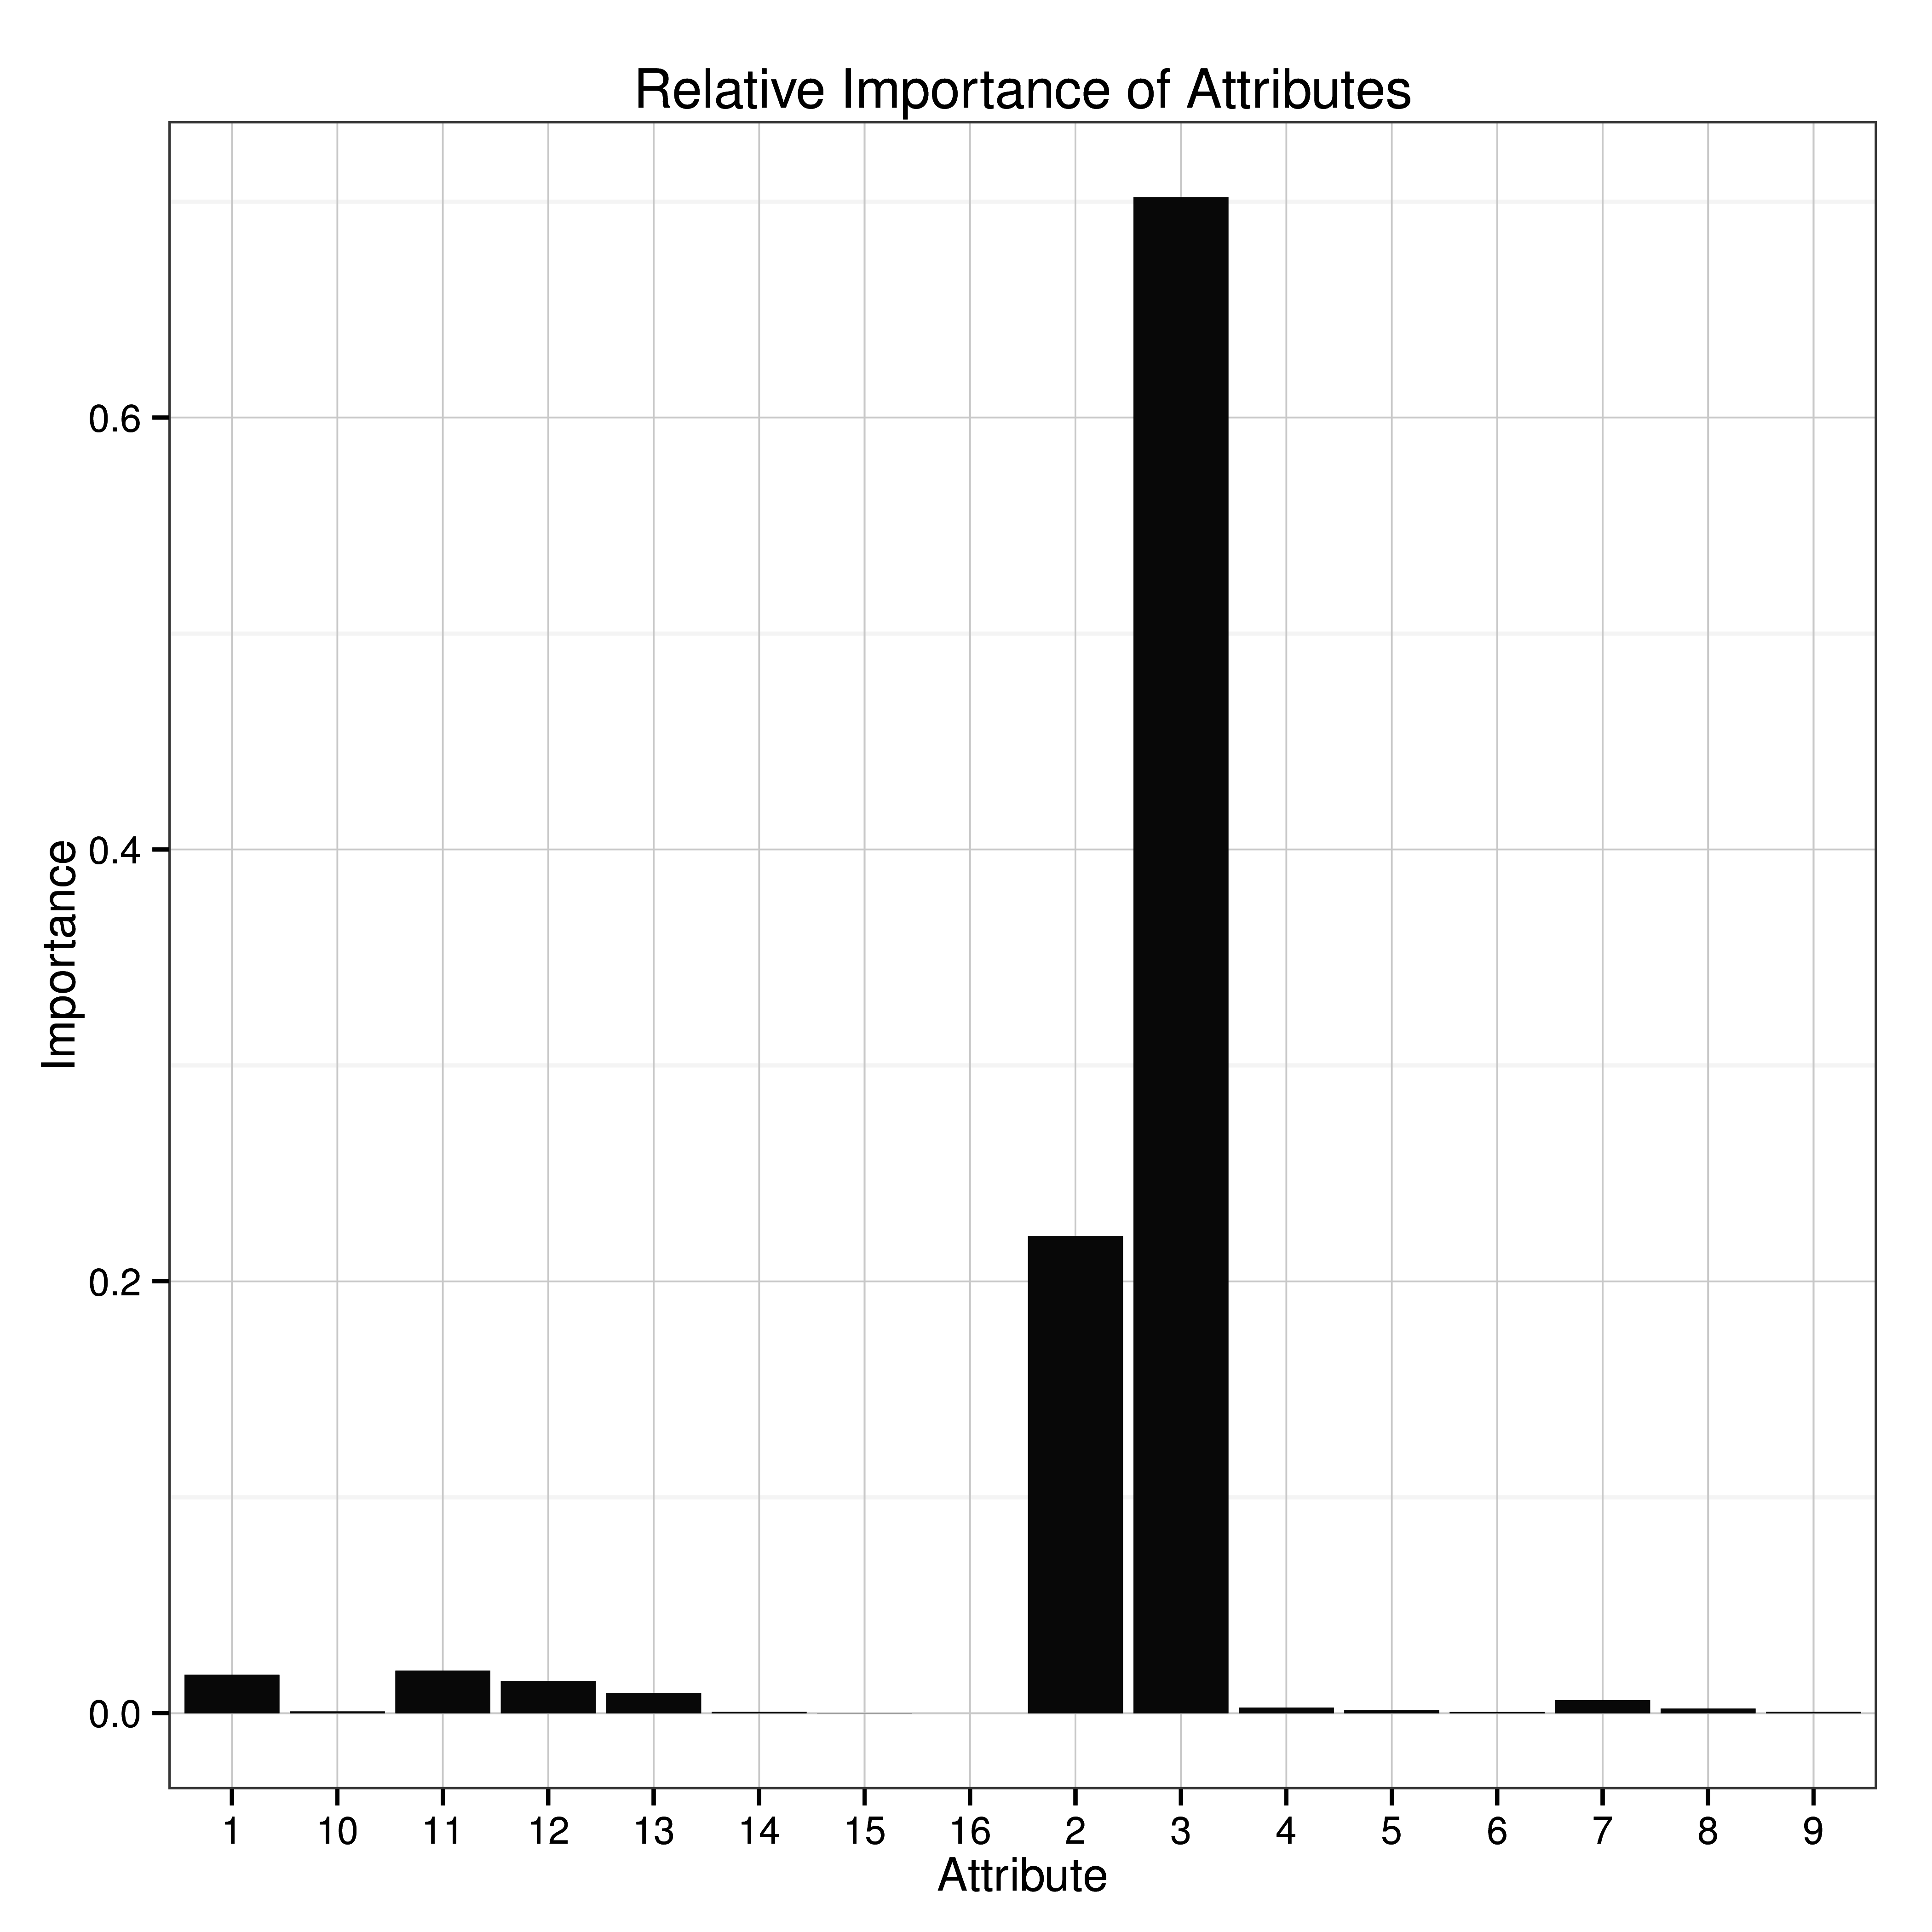
\includegraphics[width=0.5\textwidth]{interpretation.png}
  \caption{Relative importance of features in the Random Forests algorithm.}
  \label{fig:importances}
  %\vspace{-50}
\end{figure}



% subsection feature_importances (end)
% subsection comparison_with_average_baseline (end)

% section preliminary_results (end)

\section{Conclusions and Extensions}
\label{sec:conclusions}
We intend to run the experiments again with systematic full splitting on categorical attributes.
% section conclusions (end)

\section{Acknowledgements}
\label{sec:conclusions}
I would like to thank both my advisors for the opportunity to work on this problem and the time they spent to meet and discuss this work in spite of their very busy schedules!

% section conclusions (end)

%% The file named.bst is a bibliography style file for BibTeX 0.99c
\bibliographystyle{named}
\bibliography{report}

\end{document}
